%-----------------------------------------------------------------------
%                                            Prof. Dr. Walmes M. Zeviani
%                                leg.ufpr.br/~walmes · github.com/walmes
%                                        walmes@ufpr.br · @walmeszeviani
%                      Laboratory of Statistics and Geoinformation (LEG)
%                Department of Statistics · Federal University of Paraná
%                                       2019-fev-15 · Curitiba/PR/Brazil
%-----------------------------------------------------------------------

%-----------------------------------------------------------------------
% Intruções de compilação.

%-----------------------------------------------------------------------

% Classe do documento: http://ctan.math.utah.edu/ctan/tex-archive/macros/latex/contrib/sciposter/scipostermanual.pdf
\documentclass[portrait, 24pt, final]{sciposter}

%\usepackage{fancybullets}
%\usepackage{other packages you may want to use}

%\definecolor{BoxCol}{rgb}{0.9,0.9,0.9}
% uncomment for grey background to \section boxes
% for use with default option boxedsections

%\definecolor{BoxCol}{rgb}{0.9,0.9,1}
% uncomment for light blue background to \section boxes
% for use with default option boxedsections

%\definecolor{SectionCol}{rgb}{0,0,0.5}
% uncomment for dark blue \section text

%-----------------------------------------------------------------------
% Pacotes.

\usepackage[brazil]{babel}
\usepackage[utf8]{inputenc}
\usepackage{graphicx}

\usepackage{amsmath, amsfonts, amssymb, amsxtra, amsthm}
\renewcommand{\labelitemi}{\small $\blacktriangleright$}

\usepackage[mathscr]{eucal}
\usepackage{icomma}
\usepackage{color}
\usepackage{indentfirst}
\setlength{\parindent}{3cm}
\usepackage{multicol}
\usepackage{setspace}
\onehalfspace
\usepackage[hang]{caption}

\usepackage{natbib}
\bibpunct{(}{)}{;}{a}{,}{,}

\usepackage{fancybox}
\usepackage{tikz}
\usetikzlibrary{positioning, shapes, shadows, arrows}

\usepackage{Sweave}

\usepackage{lipsum}

%-----------------------------------------------------------------------

% \definecolor{BoxCol}{rgb}{0.470,0.537,0.568}
\definecolor{BoxCol}{rgb}{0.25, 0.25, 0.25}
% \definecolor{SectionCol}{rgb}{1,1,1}
\definecolor{SectionCol}{rgb}{1,0.5,0.25}

%-----------------------------------------------------------------------
\begin{document}

% Imagem de cabeçalho do poster.
\begin{tikzpicture}[remember picture, overlay]
  \node[anchor = north east, inner sep = 0em]
  % at (current page.north east)
  at (76, 5.5)
  {
\includegraphics[width = 1.0\paperwidth]{capa_texto.png}};
\end{tikzpicture}

\conference{
  \normalsize I Encontro de Data Science \& Big Data, 28 de Junho de 2019, Curitiba/PR
}

\vspace{10cm}

\noindent
\begin{minipage}[c][10cm][c]{0.75\textwidth}

  \vspace{6ex}
  {\Huge
	Nostradamus: plataforma de aprendizado de máquina como um serviço para tratamente, análise, visualização e previsão de sér    ies temporais providas pelo usuário}

  \vspace{1ex}
  {\Large
    Jayme T. Anchante$^1$,
    André R. A. Grégio$^2$,
  }

  \vspace{1ex}
  $^1${Aluno do programa de Especialização em Data Science \& Big Data, {\it jayme.anchante@disroot.org}};\\
  $^2${Professor do Departamento de Informática - DINF/UFPR, {\it gregio@ufpr.br}};\\

\end{minipage}

\vspace{3cm}

%-----------------------------------------------------------------------
% Conteúdo do poster.

\begin{multicols}{2}

\begin{abstract}
  O presente trabalho apresenta uma proposta de sistema automatizado de previsão de séries temporais chamado Nostradamus. Inicia-se o trabalho apresentando os principais conceitos de séries temporais, suas principais características e formas de tratamento. Em seguida, expôs-se o que se chamou de abordagem da estatística inferencial e de abordagem da estatística preditiva e as formas de tratamento e previsão de séries temporais de cada uma. Posteriormente, propôs-se o sistema automatizado Nostradamus, discutindo a forma de otimização e as etapas que o sistema percorre para alcançar a previsão final. No benchmark em sete bases de dados de séries temporais, o sistema Nostradamus alcançou o melhor resultado em cinco delas.

  \noindent  {\textbf{Palavras chaves:} {
      \it aprendizado de máquina, automl, séries temporais}.
  }
\end{abstract}

%-----------------------------------------------------------------------
\section*{Introdução}

\begin{itemize}
\item
	Série temporal são dados pontuais ordenados temporalmente. Apesar do tempo ser contínuo, normalmente uma série temporal envolve dados discretos, tomados em sequência de períodos igualmente espaçados e sucessivos de tempo. Além da análise de séries temporais, ou seja, métodos para extrair estatísticas úteis e outras características dos dados, outro tema bastante relevante e objeto de estudos do presente trabalho é a predição de séries temporais, processo que envolve o uso de modelos que predigam valores futuros com base em valores passados observados.

\item

	O objetivo do trabalho é a criação de um sistema automatizado de previsão de séries temporais que abstrai completamente questões técnicas como processamento dos dados, engenharia de características, modelagem, validação do resultado e realizar uma previsão que extrapole o período de amostra inicial.

\end{itemize}

\section*{Material e Métodos}

\begin{itemize}
\item
	O sistema Nostradamus pode ser definido numa função objetivo tal que
\begin{equation}
    \begin{split}
        & \min \quad MAE = f(FE(p), Algo(HP)) \\
        & \text{tal que} \qquad p <= n / 20 \\
        & \qquad \qquad \quad Algo(HP) \to Data \\
    \end{split}
\end{equation}

o objetivo é minimizar o erro absoluto médio ($MAE$ em inglês) das previsões de acordo com uma função de $FE$ que é a engenharia de características e de um $Algo$ ou algoritmo que tem $HP$ ou hiperparâmetros. A primeira restrição significa que a ordem $p$ da engenharia de características não deve exceder a vigésima parte do número de dados da série temporal. A segunda restrição afirma que os hiperparâmetros deve estar de acordo com a distribuição dos dados.

\item
Como engenharia de características, é feita uma transformação da série temporal em um processo autorregressivo \textit{AR(p)}, em que $p$ ou ordem máxima de defasagens da variável alvo utilizada

\item
Os algoritmos preditivos implementados pela plataforma são: regressão linear, \textit{elasticnet} (uma regressão linear com regularização L1 e L2), florestas aleatórias, $k$ vizinhos próximos, rede neural profunda, implementados pela biblioteca \textit{scikit-learn}; um algoritmo de impulso de gradiente extremo baseado em árvore de decisão com \textit{boosting} chamado de XGBoost.

\item
A forma de minimização é feita por meio de um processo iterativo em que a cada etapa um valor de $p$ é escolhido para a engenharia de características, assim como um dos algoritmos mencionados anteriormente com uma configuração de hiperparâmetros amostrados de forma que faça sentido com os dados obedecendo a segunda restrição.

\item
Um algoritmo de busca Bayesiana é responsável pela otimização da função objetivo. Ele funciona da seguinte maneira: inicialmente são feita $x$ iterações amostradas de forma totalmente aleatória para que o sistema gere dados, as amostragens de parâmetros são as características que serão inputadas e o erro absoluto médio é o alvo do algoritmo Bayesiano, assim após $x$ iterações, o algoritmo começará a testar espaços amostrais mais promissores de forma mais consistente, mas mantendo a busca aleatória a cada $y$ iterações para que o sistema não caia em um mínimo local.

\end{itemize} 

\vspace{6cm}

\section*{Resultados e discussões}

\begin{itemize}

\item

	As séries temporais utilizadas como \textit{benchmark} são: \textit{sunspots}, número de manchas solares por ano entre 1700 e 2008; \textit{airpassengers}, número mensal de passageiros de vôos de avião; \textit{austres}, dados residenciais trimestrais; \textit{heartrate}, frequência cardíaca; \textit{lynx}, número de linces capturados por ano no Canadá entre 1821 e 1934; \textit{wineind}, vendas de vinho da indústria australiana; e \textit{woolynrnq}, produção trimestral de lã na Austrália.

\item

	Foram separados os dez por cento dos pontos mais recentes de cada conjunto de dados como base de teste e cada algoritmo recebeu os noventa por cento de dados restantes para treinamento.

\item 

\begin{table}[!htb]
    \caption{Erro absoluto médio nos 10\% de cada série temporal utilizados para validação para a previsão de cada um dos três sistemas, Nostradamus, ARIMA e Prophet}
    \center
    \begin{tabular}{llll}
            Base & Nostradamus & ARIMA & Prophet \\
            sunspots & 18.93 & 44.41 & 45.50  \\  
            airpassengers & 88.74 & 39.35 & 57.93 \\
            austres & 41.74 & 56.43 & 115.42  \\
            heartrate & 1.64 & 2.01 & 2.16  \\
            lynx & 198.49 & 652.95 & 967.96  \\
            wineind & 5939.42 & 3817.89 & 3762.36  \\
            woolnrq & 426.8 & 427.38 & 592.50  \\
    \end{tabular}
\end{table}

\item
	No gráfico abaixo podemos ver a forma como cada sistema fez as previsões. A série temporal analisada é \textit{sunspots}. Enquanto o sistema Nostradamus tenta verdadeiramente ajustar o padrão das séries, os modelos ARIMA e Prophet optam por previsões mais "conservadoras" em torno da média dos dados. O sistema Nostradamus obtém uma performance melhor que os demais sistemas, pois possui um erro absoluto médio menor que os modelos ARIMA e Prophet.

\item
\begin{figure}[!htb]
        \centering 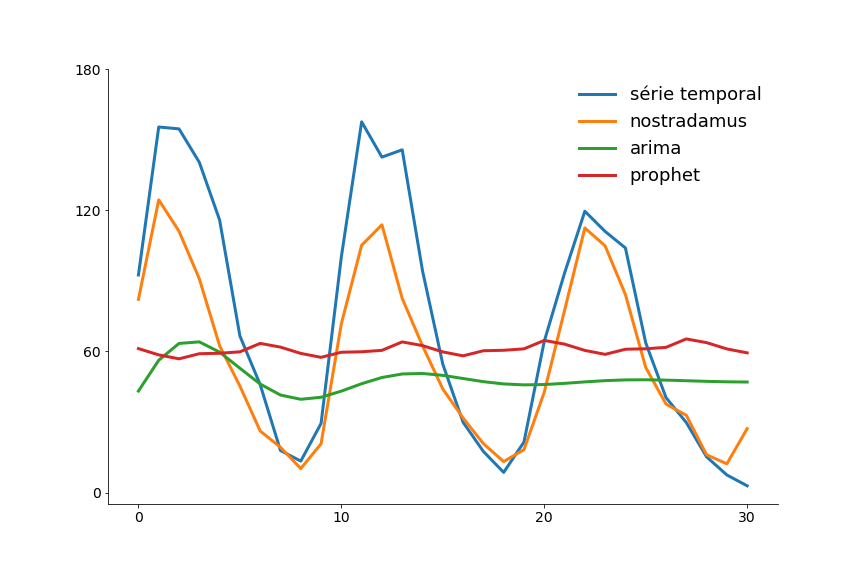
\includegraphics[scale=0.2]{fig1.png}
        \caption{Previsão de cada sistema na base \textit{sunspots} nos 10\% da base reservados para teste}
        \label{fig1}
\end{figure}

\end{itemize}

\section*{Conclusões}

Algumas conclusões preliminares alcançadas pelo trabalho são:

\begin{itemize}
\item É possível criar um sistema automatizado de previsão de séries temporais
\item O sistema Nostradamus demonstrou razoável poder preditivo frente aos demais algoritmos, alcançando a melhor performance em 5 das 7 séries temporais diversas utilizadas para \textit{benchmark}
\end{itemize}

\section*{Principais Referências}
\begin{spacing}{0.8}
\begin{itemize}
\begin{small}
 \item[] GUJARATI, D. N.; PORTER, D. \textit{Basic Econometrics}.
         5ª ed. Nova Iorque: Mc Graw-Hill/Irwin, 2009.
 \item[] PEDREGOSA, F. et al. Scikit-learn: Machine Learning in Python.
         \textit{Journal of Machine Learning Research}, v. 12, p. 2825-2830, 2011.
 \item[] CHEN, T.; GUESTRIN, C. XGBoost: A Scalable Tree Boosting System.
         In: \textit{Proceedings of the 22nd ACM SIGKDD International Conference on Knowledge Discovery and Data Mining}.
         São Francisco, CA, USA: ACM, 13-17 Agosto de 2016. p. 785–794. arXiv:1603.02754.
\end{small}
\end{itemize}
\end{spacing}

\end{multicols}
\end{document}
